%package list
\documentclass{article}
\usepackage[top=3cm, bottom=3cm, outer=3cm, inner=3cm]{geometry}
\usepackage{multicol}
\usepackage{graphicx}
\usepackage{url}
%\usepackage{cite}
\usepackage{hyperref}
\usepackage{array}
%\usepackage{multicol}
\newcolumntype{x}[1]{>{\centering\arraybackslash\hspace{0pt}}p{#1}}
\usepackage{natbib}
\usepackage{pdfpages}
\usepackage{multirow}
\usepackage[normalem]{ulem}
\useunder{\uline}{\ul}{}
\usepackage{svg}
\usepackage{xcolor}
\usepackage{listings}

\lstdefinestyle{ascii-tree}{
    literate={├}{|}1 {─}{--}1 {└}{+}1 
  }
\lstset{basicstyle=\ttfamily,
  showstringspaces=false,
  commentstyle=\color{red},
  keywordstyle=\color{blue}
}
%\usepackage{booktabs}
\usepackage{caption}
\usepackage{subcaption}
\usepackage{float}
\usepackage{array}

\newcolumntype{M}[1]{>{\centering\arraybackslash}m{#1}}
\newcolumntype{N}{@{}m{0pt}@{}}


%%%%%%%%%%%%%%%%%%%%%%%%%%%%%%%%%%%%%%%%%%%%%%%%%%%%%%%%%%%%%%%%%%%%%%%%%%%%
%%%%%%%%%%%%%%%%%%%%%%%%%%%%%%%%%%%%%%%%%%%%%%%%%%%%%%%%%%%%%%%%%%%%%%%%%%%%
\newcommand{\itemEmail}{jgordillome@unsa.edu.pe}
\newcommand{\itemStudent}{Jose Alonzo Gordillo Mendoza}
\newcommand{\itemCourse}{Programación Web 2}
\newcommand{\itemCourseCode}{20220577}
\newcommand{\itemSemester}{III}
\newcommand{\itemUniversity}{Universidad Nacional de San Agustín de Arequipa}
\newcommand{\itemFaculty}{Facultad de Ingeniería de Producción y Servicios}
\newcommand{\itemDepartment}{Departamento Académico de Ingeniería de Sistemas e Informática}
\newcommand{\itemSchool}{Escuela Profesional de Ingeniería de Sistemas}
\newcommand{\itemAcademic}{2023 - A}
\newcommand{\itemInput}{Del 08 Mayo 2023}
\newcommand{\itemOutput}{Al 15 Junio 2023}
\newcommand{\itemPracticeNumber}{05}
\newcommand{\itemTheme}{Python - Django}
%%%%%%%%%%%%%%%%%%%%%%%%%%%%%%%%%%%%%%%%%%%%%%%%%%%%%%%%%%%%%%%%%%%%%%%%%%%%
%%%%%%%%%%%%%%%%%%%%%%%%%%%%%%%%%%%%%%%%%%%%%%%%%%%%%%%%%%%%%%%%%%%%%%%%%%%%

\usepackage[english,spanish]{babel}
\usepackage[utf8]{inputenc}
\AtBeginDocument{\selectlanguage{spanish}}
\renewcommand{\figurename}{Figura}
\renewcommand{\refname}{Referencias}
\renewcommand{\tablename}{Tabla} %esto no funciona cuando se usa babel
\AtBeginDocument{%
	\renewcommand\tablename{Tabla}
}

\usepackage{fancyhdr}
\pagestyle{fancy}
\fancyhf{}
\setlength{\headheight}{30pt}
\renewcommand{\headrulewidth}{1pt}
\renewcommand{\footrulewidth}{1pt}
\fancyhead[L]{\raisebox{-0.2\height}{
\includegraphics[width=3cm]{img/logo_episunsa.png}}}
\fancyhead[C]{\fontsize{7}{7}\selectfont	\itemUniversity \\ \itemFaculty \\ \itemDepartment \\ \itemSchool \\ \textbf{\itemCourse}}
\fancyhead[R]{\raisebox{-0.2\height}{
\includegraphics[width=1.2cm]{img/logo_abet}}}
\fancyfoot[L]{Estudiante Jose Gordillo Mendoza}
\fancyfoot[C]{\itemCourse}
\fancyfoot[R]{Página \thepage}

% para el codigo fuente
\usepackage{listings}
\usepackage{color, colortbl}
\definecolor{dkgreen}{rgb}{0,0.6,0}
\definecolor{gray}{rgb}{0.5,0.5,0.5}
\definecolor{mauve}{rgb}{0.58,0,0.82}
\definecolor{codebackground}{rgb}{0.95, 0.95, 0.92}
\definecolor{tablebackground}{rgb}{0.8, 0, 0}

\lstset{frame=tb,
	language=bash,
	aboveskip=3mm,
	belowskip=3mm,
	showstringspaces=false,
	columns=flexible,
	basicstyle={\small\ttfamily},
	numbers=none,
	numberstyle=\tiny\color{gray},
	keywordstyle=\color{blue},
	commentstyle=\color{dkgreen},
	stringstyle=\color{mauve},
	breaklines=true,
	breakatwhitespace=true,
	tabsize=3,
	backgroundcolor= \color{codebackground},
}

\begin{document}
	
	\vspace*{10px}
	
	\begin{center}	
		\fontsize{17}{17} \textbf{ Informe de Laboratorio \itemPracticeNumber}
	\end{center}
	\centerline{\textbf{\Large Tema: \itemTheme}}
	%\vspace*{0.5cm}	

	\begin{flushright}
		\begin{tabular}{|M{2.5cm}|N|}
			\hline 
			\rowcolor{tablebackground}
			\color{white} \textbf{Nota}  \\
			\hline 
			     \\[30pt]
			\hline 			
		\end{tabular}
	\end{flushright}	

	\begin{table}[H]
		\begin{tabular}{|x{4.7cm}|x{4.8cm}|x{4.8cm}|}
			\hline 
			\rowcolor{tablebackground}
			\color{white} \textbf{Estudiante} & \color{white}\textbf{Escuela}  & \color{white}\textbf{Asignatura}   \\
			\hline 
			{\itemStudent \par \itemEmail} & \itemSchool & {\itemCourse \par Semestre: \itemSemester \par Código: \itemCourseCode}     \\
			\hline 			
		\end{tabular}
	\end{table}		
	
	\begin{table}[H]
		\begin{tabular}{|x{4.7cm}|x{4.8cm}|x{4.8cm}|}
			\hline 
			\rowcolor{tablebackground}
			\color{white}\textbf{Laboratorio} & \color{white}\textbf{Tema}  & \color{white}\textbf{Duración}   \\
			\hline 
			\itemPracticeNumber & \itemTheme & 04 horas   \\
			\hline 
		\end{tabular}
	\end{table}
	
	\begin{table}[H]
		\begin{tabular}{|x{4.7cm}|x{4.8cm}|x{4.8cm}|}
			\hline 
			\rowcolor{tablebackground}
			\color{white}\textbf{Semestre académico} & \color{white}\textbf{Fecha de inicio}  & \color{white}\textbf{Fecha de entrega}   \\
			\hline 
			\itemAcademic & \itemInput &  \itemOutput  \\
			\hline 
		\end{tabular}
	\end{table}
	
	\section{Tarea}
	\begin{itemize}		
		\item Crea un blog sencillo en un entorno virtual utilizando la guía: \url{https://tutorial.djangogirls.org/es/django_start_project/}
            \item Especificar paso a paso la creación del blog en su informe.
	\end{itemize}
        \begin{figure}[H]
		\centering
		
\includegraphics[width=0.25\textwidth,keepaspectratio]{img/django.png}
	\end{figure}

	\section{URL de Repositorio Github}
	\begin{itemize}
		\item URL para el laboratorio 05 en el Repositorio GitHub.
		\item \url{https://github.com/JoseGordilloMendoza/lab05-PW2.git}
	\end{itemize}
	
	\section{Ejercicios}
 
        \subsection{Estructura de laboratorio 05}
	\begin{itemize}	
		\item La distribucion de archivos sera la siguiente (teniendo en cuenta solo el entorno virtual y los archivos mas importantes, por ejemplo lo descargado en el entorno es demasiado extense como para incluirlo, el latex y un README estaran en la carpeta anterior):
	\end{itemize}
	
\begin{lstlisting}[style=ascii-tree]
lab05-PW2/
    ├──lab05/
        ├── blog
            ├── __pycache__
            ├── migrations
            ├── static
                ├── css
                    ├── blog.css
            ├── templates
                ├── blog
                    ├── base.html
                    ├── post_detail.html
                    ├── post_edit.html
                    ├── post_list.html
            ├── __init__.py
            ├── admin.py
            ├── apps.py
            ├── forms.py
            ├── models.py
            ├── tests.py
            ├── urls.py
            ├── views.py
        ├── Lib
        ├── mysite
            ├── __pycache__
            ├── __init__.py
            ├── settings.py
            ├── urls.py
            ├── wsgi.py
        ├── Scripts
        ├── db.sqlite3
        ├── manage.py
        ├── pyvenv.cfg

\end{lstlisting}  
 
	\subsection{Análisis de archivos }
 
        \begin{itemize}	
		\item En primer lugar hay que hablar del entorno virtual, que como vimos en la clase pasada, nos ayudara a crear nuestra blog en este caso:\newline\newline
    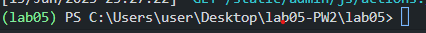
\includegraphics[width=15cm]{img/Entorno virtual.png}
	\end{itemize}
        
	\begin{lstlisting}[language=bash,caption={Analizando bloque 1 de settings.py}][H]
            INSTALLED_APPS = [
                'django.contrib.admin',
                'django.contrib.auth',
                'django.contrib.contenttypes',
                'django.contrib.sessions',
                'django.contrib.messages',
                'django.contrib.staticfiles',
                'blog.apps.BlogConfig',
            ]
	\end{lstlisting}
        Estas son las configuraciones de las aplicaciones instaladas, la ultima aplicacion "blog" es la que creamos para nuestro blog personal.
                  
	\begin{lstlisting}[language=bash,caption={Settings.py - cambio de idioma y region}][H]
            LANGUAGE_CODE = 'es-es'
            TIME_ZONE = 'America/Lima'
	\end{lstlisting}
        En este bloque vemos como hemos modificado el idioma que se manejara asi como la region que eran originalmente ingles y UTC respectivamente.

        \begin{lstlisting}[language=bash,caption={Settings.py - cambio 3}][H]
            STATIC_URL = 'static/'
            STATIC_ROOT = BASE_DIR / 'static'
	\end{lstlisting}
        Se agrego la ultima linea al "settings.py" original para especificar la ubicación de la carpeta raíz donde se almacenarán los archivos estáticos recopilados en el proyecto.
        
        \begin{itemize}	
    		\item Una vez modificado esto veamos la aplicacion "blog" creada a traves del comando "python manage.py startapp blog" que crea un nuevo directorio; por tanto analicemos en primer lugar a "models.py"
        \end{itemize}
        \begin{lstlisting}[language=bash,caption={bloque4}][H]
        from django.conf import settings
        from django.db import models
        from django.utils import timezone
        
        class Post(models.Model):
            author = models.ForeignKey(settings.AUTH_USER_MODEL, on_delete=models.CASCADE)
            title = models.CharField(max_length=200)
            text = models.TextField()
            created_date = models.DateTimeField(
                    default=timezone.now)
            created_date = models.DateTimeField(
                    blank=True, null=True)
        
            def publish(self):
                self.published_date = timezone.now()
                self.save()
        
            def __str__(self):
                return self.title
	\end{lstlisting}
    Este es nuestro modelo Post, antes de verlo mejor, tengamos en cuenta las importaciones que hacemos del mismo django, usando sus modelos y el timezone especialmente para obtener
    la fecha actual; entonces veamos que se tienen los atributos author, title, created\_date  y created\_date para definir sus respectivos aspectos usando al usuario que inicio sesion, un titulo y texto a ingresar, la hora de creacion; ademas de metodos que publicaran/guardaran los posts y nos devolveras el titulo de objeto como representacion.

        \begin{itemize}	
    		\item Archivo admin
        \end{itemize}
        
        \begin{lstlisting}[language=bash,caption={admin.py}][H]
            from django.contrib import admin

            from django.contrib import admin
            from .models import Post
            
            admin.site.register(Post)
	\end{lstlisting}
    Como vemos importamos el modelo Post antes presentado, y se registra en la interfaz de administración de Django. Esto permitirá que el modelo Post sea administrado y se pueda crear, editar y eliminar instancias de Post a través de la interfaz de administración. Para iniciar sesión, se debera crear un superusuario (superuser), con la linea de comando "manage.py createsuperuser".

        \begin{itemize}	
    		\item Archivo urls
        \end{itemize}
        
        \begin{lstlisting}[language=bash,caption={urls.py}][H] 
            from django.urls import path
            from . import views
            
            urlpatterns = [
                path('', views.post_list, name='post_list'),
                path('post/<int:pk>/', views.post_detail, name='post_detail'),
                path('post/new', views.post_new, name='post_new'),
                path('post/<int:pk>/edit/', views.post_edit, name='post_edit'),
                path('delete_post/<int:id>', views.deletePost, name = "delete_post")
            ]
	\end{lstlisting}
    Estas son las rutas que usaremos en nuestro blog, la primera siendo la ruta raiz o la pagina principal, la segunda ruta se utiliza para mostrar detalles de un post específico, la tercer ruta se encargará de mostrar el formulario de creación de un nuevo post, luego la cuarta que se utilizara  para editar un post existente y la ultima con la que borraremos el post.

	\begin{itemize}	
		\item Archivos views
	\end{itemize}
	\begin{lstlisting}[language=bash,caption={Primer parte de views.py}][H]
            def post_list(request):
                posts= Post.objects.filter(published_date__lte=timezone.now()).order_by('published_date')
                return render(request, 'blog/post_list.html', {'posts': posts})
            
            def post_detail(request, pk):
                post = get_object_or_404(Post, pk=pk)
                return render(request, 'blog/post_detail.html', {'post': post})
            
            def post_new(request):
                if request.method == "POST":
                    form = PostForm(request.POST)
                    if form.is_valid():
                        post = form.save(commit=False)
                        post.author = request.user
                        post.published_date = timezone.now()
                        post.save()
                        return redirect('post_detail', pk=post.pk)
                else:
                    form = PostForm()
                return render(request, 'blog/post_edit.html', {'form': form})
	\end{lstlisting}
        En primer lugar post\_list  maneja la vista de la lista de publicaciones en el blog. Filtra las publicaciones por fecha de publicación anterior o igual a la fecha y hora actual, luego, ordena las publicaciones por fecha de publicación ascendente , para luego pasarlas publicaciones filtradas como contexto.
        Por otra parte post\_detail maneja la vista de detalle de una publicación específica en el blog. Por ultimo post\_new maneja la vista para crear una nueva publicación en el blog. Si la solicitud es de tipo POST, se crea una instancia de PostForm con los datos proporcionados en la solicitud. Luego, se verifica si el formulario es válido utilizando. Si es válido, se guarda la instancia de Post. Se establece el autor de la publicación como el usuario actual  y la fecha de publicación como la fecha y hora actual. Finalmente, se guarda la publicación y se redirige a la vista de detalle de la publicación creada. Si la solicitud no es de tipo POST, se crea una instancia vacía de PostForm.

	\begin{lstlisting}[language=bash,caption={Segunda parte de views.py}][H]
        def post_edit(request, pk):
            post = get_object_or_404(Post, pk=pk)
            if request.method == "POST":
                form = PostForm(request.POST, instance=post)
                if form.is_valid():
                    post = form.save(commit=False)
                    post.author = request.user
                    post.published_date = timezone.now()
                    post.save()
                    return redirect('post_detail', pk=post.pk)
            else:
                form = PostForm(instance=post)
            return render(request, 'blog/post_edit.html', {'form': form})

        def deletePost(request, id):
            post = Post.objects.get(id=id)
            post.delete()
            return redirect('/')
	\end{lstlisting}
        Esta funcion post\_edit maneja la vista para editar una publicación existente en el blog. Toma como argumentos la solicitud (request) y el parámetro pk que representa la clave primaria de la publicación que se desea editar, en esta se obtiene una instancia de la publicación específica, si la publicación no existe, se devuelve una página de error 404.Dentro del bloque if, se crea una instancia de PostForm con los datos enviados en la solicitud. Se utiliza el argumento instance=post para vincular el formulario con la instancia de la publicación que se está editando.
        Se verifica si el formulario es válido . Si es válido, se guardan los cambios en la instancia de Post. Luego, se guarda la publicación y se redirige a la vista de detalle de la publicación editada.
        Si la solicitud no es de tipo POST, se crea una instancia de PostForm con los datos de la publicación existente. Es decir, esta función permite editar una publicación existente en el blog.
        La ultima funcion "deletePost"elimina un objeto Post de la base de datos según el id proporcionado y redirige al usuario a la página principal del blog.

        \begin{itemize}	
		\item Plantilas HTML (haremos uso de variables con llaves, asi como el extenderse de archivos que srivan como base)
	\end{itemize}
	\begin{lstlisting}[language=bash,caption={base.html}][H]
            
            <html>
                <head>
                    <title>BLOG</title>
                    <link rel="stylesheet" href="//maxcdn.bootstrapcdn.com/bootstrap/3.2.0/css/bootstrap.min.css">
                    <link rel="stylesheet" href="//maxcdn.bootstrapcdn.com/bootstrap/3.2.0/css/bootstrap-theme.min.css">
                    <link href='//fonts.googleapis.com/css?family=Lobster&subset=latin,latin-ext' rel='stylesheet' type='text/css'>
                    <link rel="stylesheet" href="">
                </head>
                <body>
                    <div class="page-header">
                        <a href="" class="top-menu"><span class="glyphicon glyphicon-plus"></span></a>
                        <h1><a href="/">MI PRIMER BLOG EN DJANGO</a></h1>
                    </div>
                    <div class="content container">
                        <div class="row">
                            <div class="col-md-8">
                            
                            
                            </div>
                        </div>
                    </div>
                </body>
            </html>
	\end{lstlisting}
        Esta plantilla HTML proporciona una estructura básica para las páginas del blog. Define un encabezado con un enlace para crear una nueva publicación y un título del blog, y proporciona una estructura de columnas para el contenido principal. 

        \begin{lstlisting}[language=bash,caption={post\_detail.html}][H]
            
            
                <div class="post">
                    
                        <div class="date">
                            {{ post.published_date }}
                        </div>
                    
                    
                        <a class="btn btn-default" href=""><span class="glyphicon glyphicon-pencil"></span></a>
                    
                    <h2>{{ post.title }}</h2>
                    <p>{{ post.text|linebreaksbr }}</p>
                </div>
            
	\end{lstlisting}
         En esta plantilla vemos que se extiende (extends) la plantilla base y define el contenido específico para la página de detalle de una publicación de blog. Muestra la fecha de publicación (si está disponible), un botón de edición para usuarios autenticados, el título de la publicación y el texto de la publicación con saltos de línea convertidos en elementos HTML <br>.

        \begin{lstlisting}[language=bash,caption={post\_edit.html}][H]
            
            
                <h2>New post</h2>
                <form method="POST" class="post-form"> 
                    {{ form.as_p }}
                    <button type="submit" class="save btn btn-default">Guardar</button>
                </form>
            
	\end{lstlisting}
         Esta plantilla extiende la plantilla base nuevamente y define el contenido específico para la página de creación de una nueva publicación en el blog. Muestra un encabezado "New post" seguido de un formulario que permite al usuario ingresar los detalles de la nueva publicación y guardarla al hacer clic en el botón "Guardar".

         \begin{lstlisting}[language=bash,caption={post\_list.html}][H]
            
                
                    
                        <div class="post">
                            <div class="date">
                                {{ post.published_date }}
                            </div>
                            <h2><a href="">{{ post.title }}</a></h2>
                            <p>{{ post.text|linebreaksbr }}</p>
                        </div>
                    
                
	\end{lstlisting}
        Esta plantilla tambien extiende la plantilla base y define el contenido específico para la página de lista de publicaciones del blog. Utiliza un bucle para mostrar cada publicación individualmente. Cada publicación se muestra con su fecha de publicación, título (como un enlace a la página de detalle de la publicación) y texto.

        \item \textbf{Archivos de estilos, blogs.css}
        \begin{lstlisting}[language=bash,caption={blog.css}][H]
            .page-header {
                background-color: #C25100;
                margin-top: 0;
                padding: 20px 20px 20px 40px;
            }
            .page-header h1, .page-header h1 a, .page-header h1 a:visited, .page-header h1 a:active {
                color: #ffffff;
                font-size: 36pt;
                text-decoration: none;
            }
            .content {
                margin-left: 40px;
            }
            h1, h2, h3, h4 {
                font-family: 'Impact', cursive;
            }
            .date {
                color: #828282;}
            .save {
                float: right;}
            
            .post-form textarea, .post-form input {
                width: 100%;}
            .top-menu, .top-menu:hover, .top-menu:visited {
                color: #ffffff;
                float: right;
                font-size: 26pt;
                margin-right: 20px;}
            .post {
                margin-bottom: 70px; }
            
            .post h2 a, .post h2 a:visited {
                color: #000000;
            }
	\end{lstlisting}
        Estos son los estilos que se usaron en el blog, que usan adicionalmente BootStrap; lo importante es mencionar que este es un archivo estatico, que maneja clases de los html anteriormente vistos.

        \item \textbf{Archivo forms}
        \begin{lstlisting}[language=bash,caption={forms.py}][H]
            from django import forms
            from .models import Post
            
            class PostForm(forms.ModelForm):
            
                class Meta:
                    model = Post
                    fields = ('title', 'text',)
            }
	\end{lstlisting}
        Este bloque de código define un formulario llamado PostForm que se utiliza para crear o editar una publicación en el blog. El formulario está vinculado al modelo Post y contiene los campos title y text. Este formulario facilita la creación y edición de publicaciones en el blog al proporcionar un conjunto de campos predefinidos y lógica de validación integrada.\newline\newline
        \subsection{Demostracion de pagina}
        Ahoa veamos a la pagina como tal:\newline\newline
        \textbf{Primero tenemos que correr nuestro server con el comando "python manage.py runserver", una vez dentro veamos la pantall principal:} \newline \newline \newline \newline 
        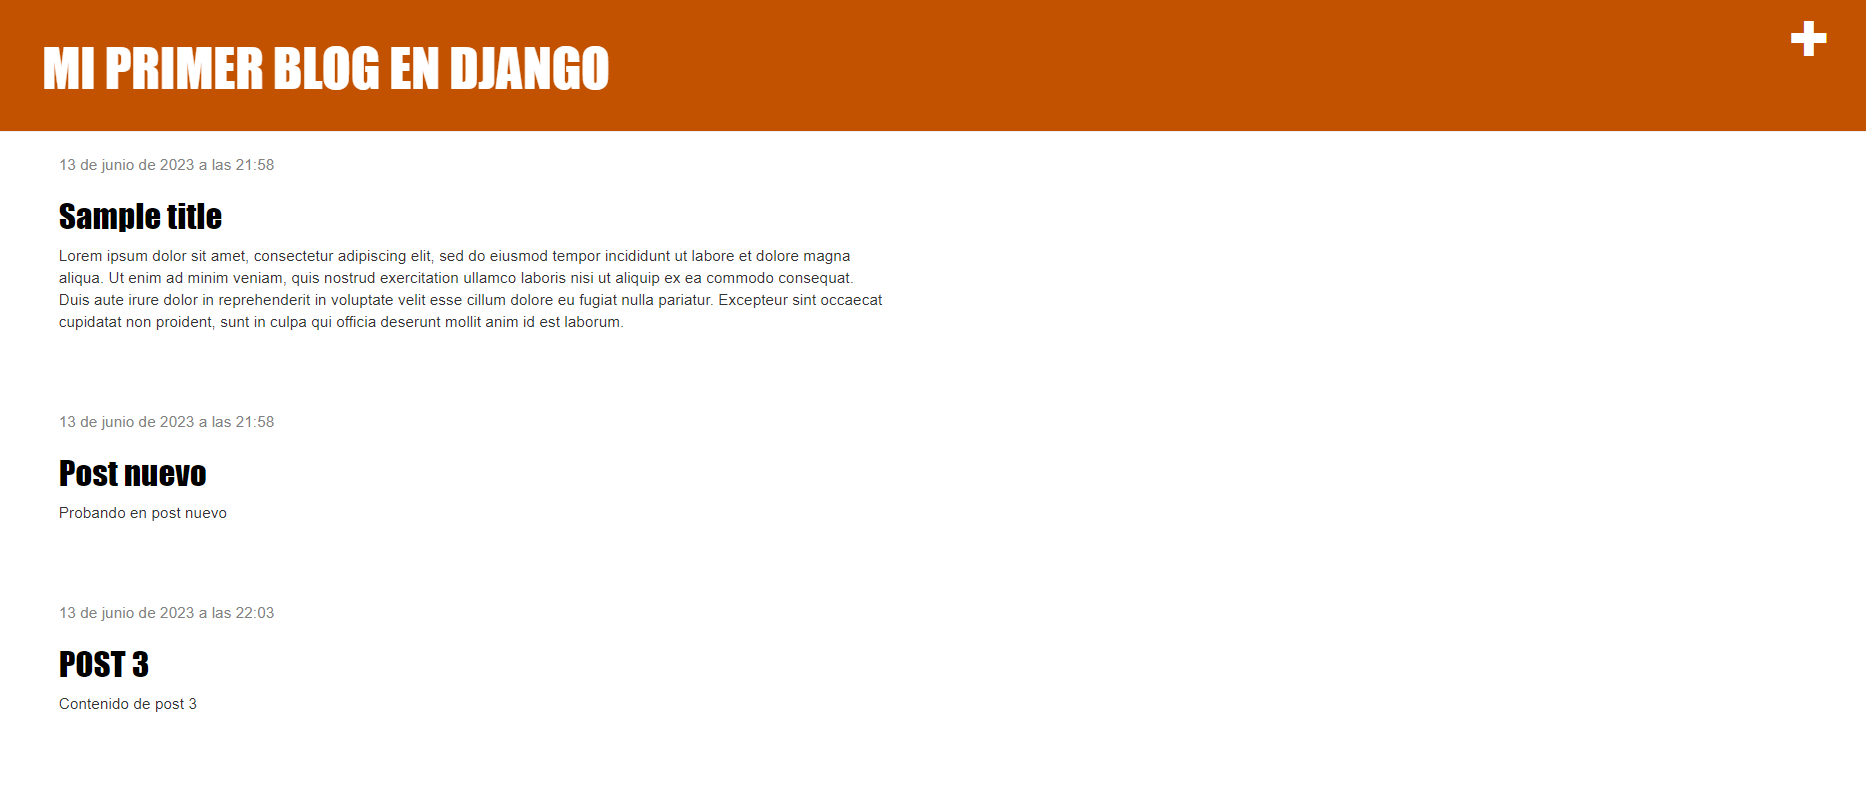
\includegraphics[width=16cm]{img/paginaInicial.png}
        Como vemos tenemos tres posts iniciales y un boton para poder agregar mas posts, pero si queremos entrar a un post, simplemente le damos en su titulo:
        \newline\newline
        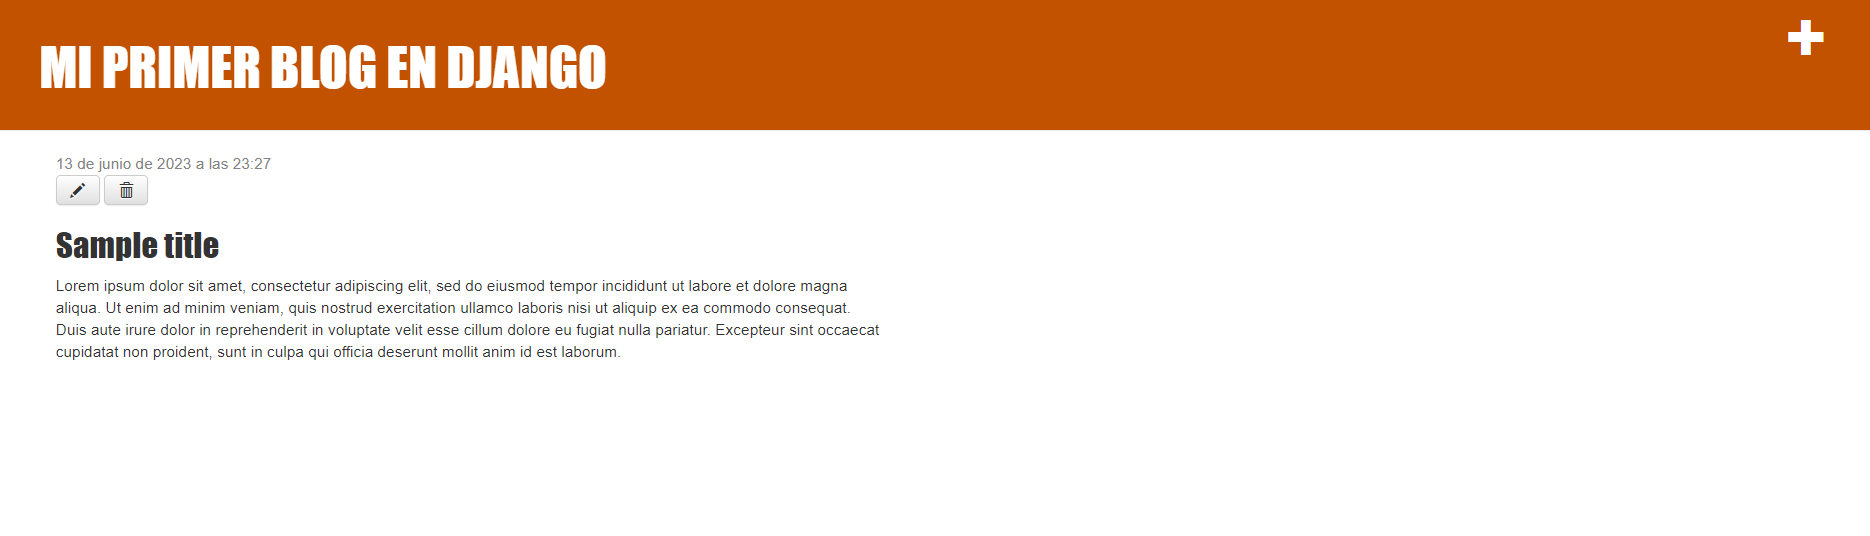
\includegraphics[width=16cm]{img/detallesPOST.png}
        Esta es la vista que tenemos de un post especifico, como vemos tenemos un lapicito con el que podemos editar el post, siempre y cuando seamos un usuario verificado y dueño del post, a su derecha hay un tacho que es para eliminar el post siguiendo la misma logica de estar "logeado":
        \newline\newline
        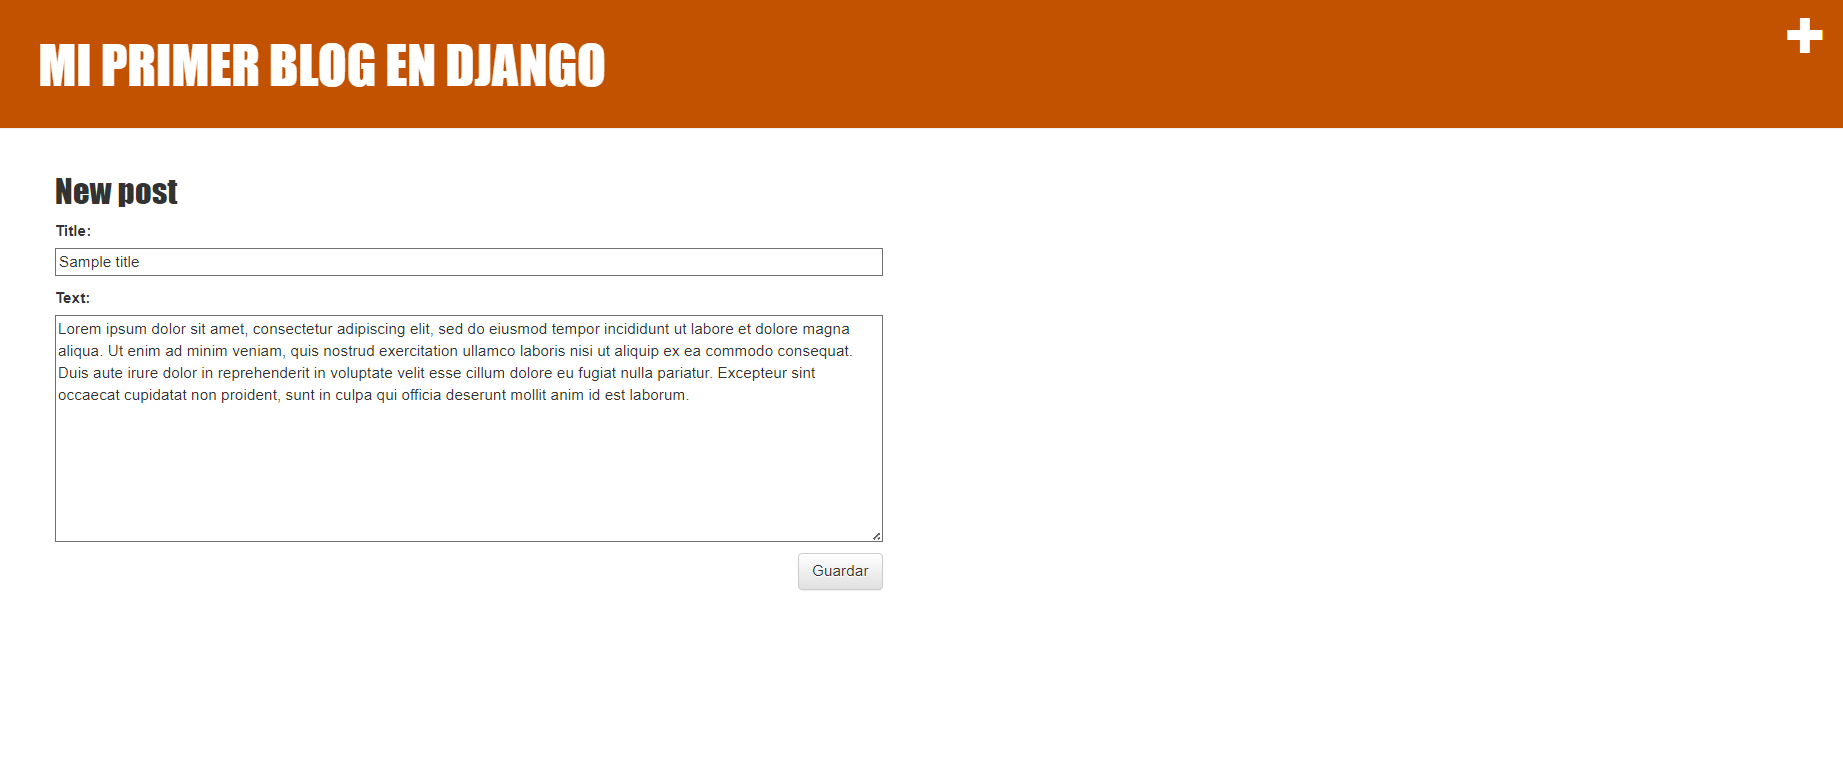
\includegraphics[width=16cm]{img/edicionPosts.png}
        \newline\newline\newline
        Ahora veamos en el apartado de administrador nuestro usuario:
        \newline\newline
        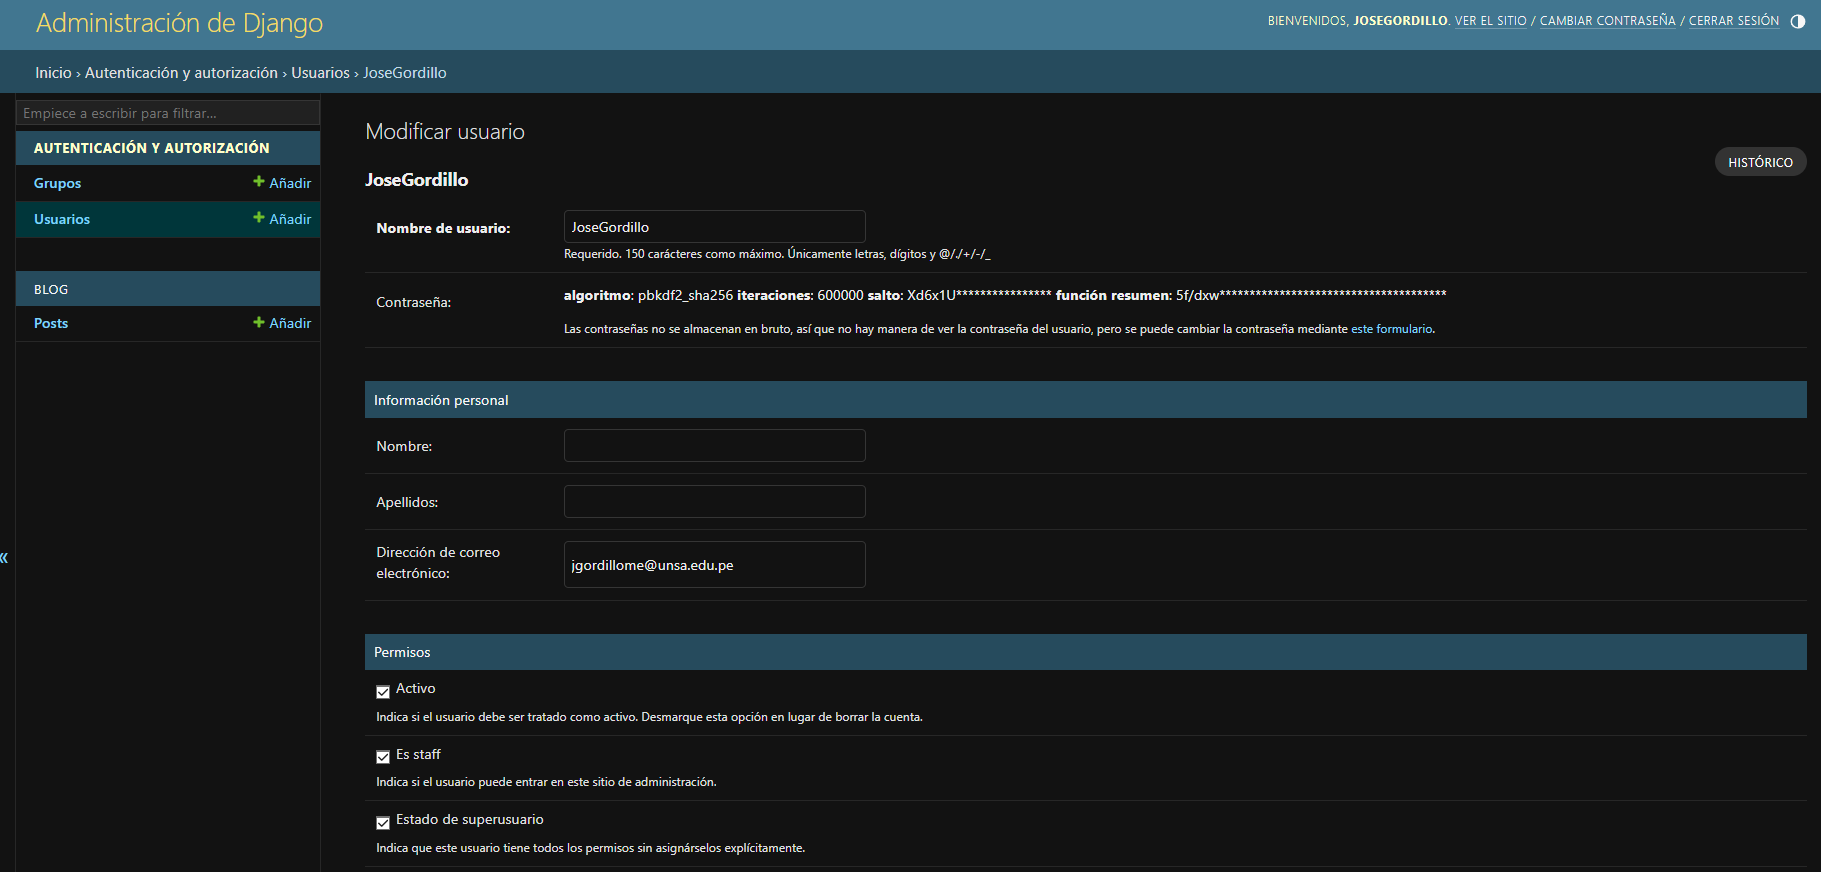
\includegraphics[width=16cm]{img/USUARIO.png}
        Ademas tenemos los posts que se han ido creando:\newline
    
        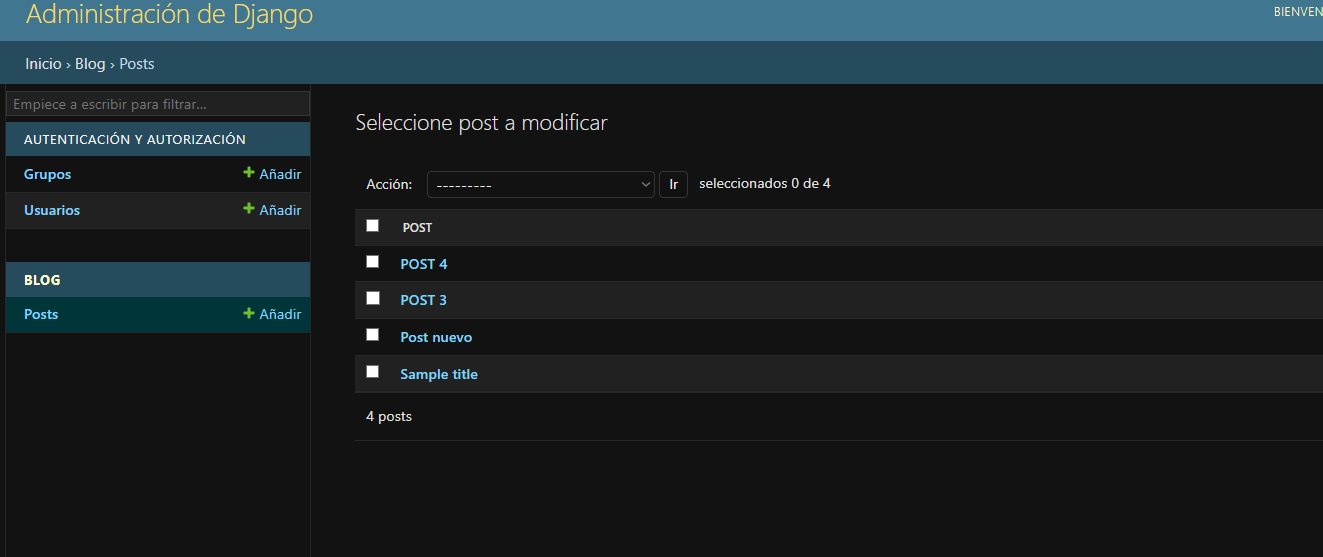
\includegraphics[width=16cm]{img/LISTADOposts.png}
        \newline\newline
        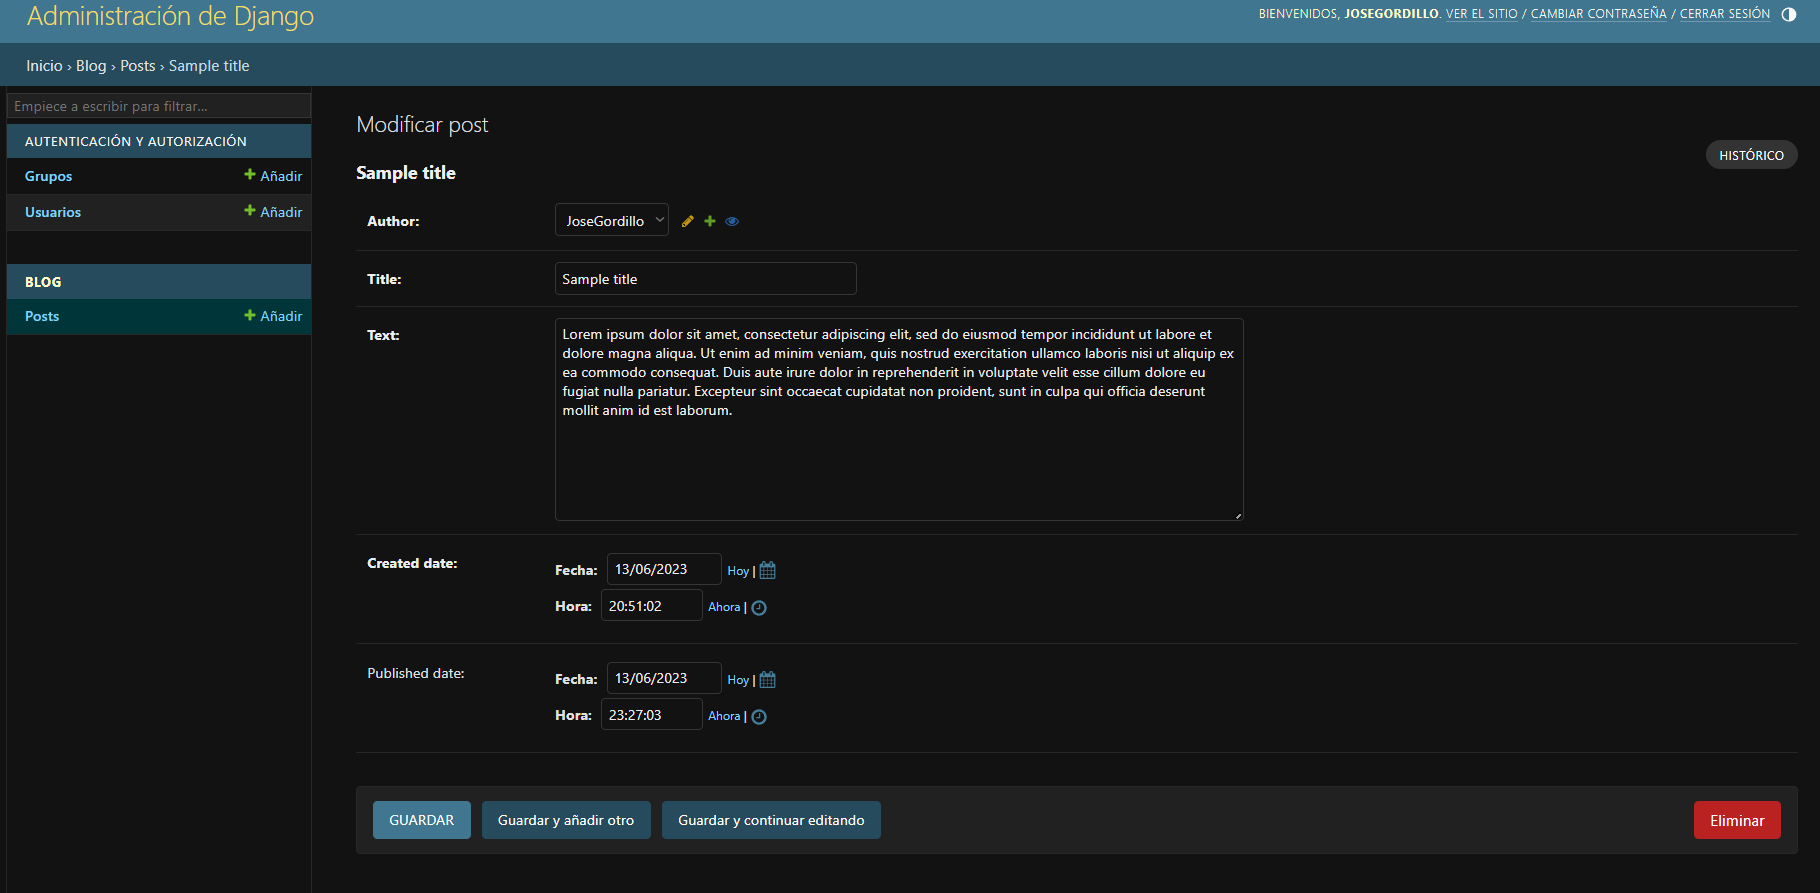
\includegraphics[width=16cm]{img/POSTejemplo.png}
        \newline
        Link donde esta alojado el video (FlipGrid): \url{https://flip.com/groups/14644257/topics/36914916/responses}
        
\section{Cuestionario}
	\begin{itemize}
		\item{¿Cuál es un estándar de codificación para Python? Ejemplo: Para PHP en el proyecto Pear \url{https://pear.php.net/manual/en/standards.php}}
        Uno de los estándares de codificación más ampliamente aceptados y utilizados en Python se conoce como PEP 8 (Python Enhancement Proposal 8). PEP 8 establece una guía de estilo para escribir código Python con el fin de mejorar la legibilidad y fomentar la coherencia entre proyectos.Estos son algunos ejemplos de las recomendaciones del PEP 8:\newline
        \textbf{- Convenciones de nomenclatura}\newline
        Usar snake\_case para nombres de variables y nombres de funciones.\newline
        CamelCase debe usarse para nombres de clase.\newline
        Hacer uso de MAYUSCULAS\_PARA\_CONSTANTES.\newline
        \textbf{- Identado y espacio:}\newline
        Usar cuatro espacios en lugar de representaciones tabulares para la sangría.\newline
        No exceder los 79 caracteres por línea de código.\newline
        Dejar dos líneas en blanco entre las definiciones de clases y funciones.\newline
         \textbf{- Importaciones:}\newline
        Completar las importaciones en líneas separadas para cada módulo.\newline
        Evitat importar varios elementos en la misma línea.\newline
         \textbf{- Comentarios:}\newline
Utilizar comentarios para explicar el código de manera concisa y clara.\newline
Evitar hacer comentarios redundantes o innecesarios.\newline

		\item{¿Qué diferencias existen entre EasyInstall, pip, y PyPM?}\newline
    EasyInstall, pip y PyPM son herramientas utilizadas en el ecosistema de Python para la instalación y gestión de paquetes. EasyInstall fue una herramienta popular en versiones antiguas de Python, pero ha sido reemplazada por pip, que es la herramienta de facto estándar en la comunidad de Python. Pip permite instalar paquetes de Python desde el registro PyPI y otros repositorios, además de gestionar dependencias y actualizaciones de paquetes de manera sencilla. Por otro lado, PyPM es una herramienta utilizada específicamente en el lenguaje Perl, no está relacionada con el sistema de paquetes de Python y tiene funcionalidades y objetivos diferentes.\newline
    En resumen EasyInstall es una herramienta de instalación y gestión de paquetes obsoleta, pip es la herramienta estándar de facto para instalar paquetes en Python, y PyPM es una herramienta utilizada específicamente para el lenguaje Perl.\newline

\item{En un proyecto Django que se debe ignorar para usar git. Vea: \url{https://github.com/django/django/blob/main/.gitignore}. ¿Qué otros tipos de archivos se deberían agregar a este archivo?}\newline
  El archivo .gitignore en un proyecto Django generalmente se utiliza para especificar los archivos y directorios que no se deben incluir en el repositorio Git. Esto ayuda a evitar que se suban al repositorio archivos innecesarios o sensibles que no deben ser compartidos públicamente.Algunos otros tipos de archivos que generalmente se deben agregar al archivo .gitignore en un proyecto Django:\newline

\textbf{- Archivos de configuración local:} Esto puede incluir archivos de configuración utilizados para almacenar datos sensibles como claves secretas, contraseñas de base de datos, etc.\newline 

\textbf{- Archivos generados automáticamente: }Estos archivos generados no son esenciales para el repositorio y pueden ser excluidos. \newline

\textbf{- Directorios y archivos estáticos generados: }Los archivos generados, como archivos CSS compilados o archivos minificados, no necesitan estar en el repositorio y pueden ser excluidos. \newline

\textbf{- Archivos de entorno:} Si se utiliza un archivo de entorno (por ejemplo, .env) para configurar variables de entorno o configuraciones específicas del entorno.\newline

\textbf{- Archivos de registro:} por ejemplo, *.log, para evitar que se llenen con registros de desarrollo o registros confidenciales.\newline
  \item{Utilice python manage.py shell para agregar objetos. ¿Qué archivos se modificaron al agregar más objetos?}\newline
  Los archivos que se modifcaron son:\newline
  \textbf{Archivo de migraciones (migrations/):} Se generaron archivos de migración en la carpeta migrations/. Estos archivos contienen instrucciones para aplicar los cambios en la base de datos y reflejar la adición de nuevos objetos o campos en el modelo. \newline

\textbf{Archivo de base de datos (db.sqlite3, postgresql, etc.):} En mi caso se usa SQLite, entonces al agregar objetos en la consola de Django, los datos se almacenarán en la base de datos. Por lo tanto, el archivo de la base de datos se modificará para incluir los nuevos registros correspondientes a los objetos agregados.
  
	\end{itemize}	
 \newpage
 \section{Conclusiones}
	\begin{itemize}
		\item  Django es un marco de desarrollo web poderoso y de alto nivel que ofrece una amplia gama de características y funcionalidades para crear aplicaciones web complejas.
		\item Django se destaca por su enfoque en la eficiencia y la seguridad, ofreciendo funciones integradas para proteger las aplicaciones web contra amenazas comunes y brindando un rendimiento efectivo y escalable.
		\item La comunidad de Django está activa y ofrece una amplia gama de recursos, documentación y paquetes complementarios.
            \item Django es un marco flexible y escalable que se puede ajustar para satisfacer las diversas necesidades y requisitos del proyecto. Es posible utilizarlo para desarrollar aplicaciones web de cualquier tamaño, desde pequeñas aplicaciones hasta proyectos empresariales de gran escala.
	\end{itemize}	
\clearpage

\section{Referencias}
\begin{itemize}	
    \item \url{https://www.w3schools.com/python/python_reference.asp}
    \item \url{ https://docs.python.org/3/tutorial/}
    \item \url{https://developer.mozilla.org/es/docs/Learn/Server-side/Django/Models}
    \item \url{https://tutorial.djangogirls.org/es/django_models/}
    \item \url{https://pear.php.net/manual/en/standards.php}
    \item \url{https://docs.djangoproject.com/en/4.0/}
    \item \url{https://www.youtube.com/watch?v=M4NIs4BM1dk}
    \item \url{https://pypi.org/}
    \item \url{https://pip.pypa.io/en/latest/user_guide/}
    \item \url{https://packaging.python.org/en/latest/tutorials/installing-packages/}
\end{itemize}	
	
%\clearpage
%\bibliographystyle{apalike}
%\bibliographystyle{IEEEtranN}
%\bibliography{bibliography}
			
\end{document}